\documentclass[tikz]{standalone}

\usepackage{tikz}
\usetikzlibrary{trees}
\usetikzlibrary{shapes}
\usetikzlibrary{positioning}
\usetikzlibrary{arrows.meta}

\tikzset{
    pointer/.style = {thick,draw=black,triangle 45-*,shorten >=-3pt},
    cell/.style = {rectangle, thick, draw=black,minimum width = 1cm, minimum height =1.0cm,fill=yellow!20},
    mynode/.style = {circle, thick, draw=black, align=center,fill=yellow!40,font=\ttfamily\bfseries\Large},
    mynoder/.style = {circle, thick, draw=black, align=center,fill=red!30,font=\ttfamily\bfseries\Large},
    mynodeb/.style = {circle, thick, draw=black, align=center,fill=blue!30,font=\ttfamily\bfseries\Large},
    edgen/.style = {-latex,ultra thick},
    edger/.style = {-latex,ultra thick,red},
    edgeb/.style = {-latex,ultra thick,blue},
    edgeg/.style = {-latex,ultra thick,gray},
    edgegd/.style = {-latex,ultra thick,brown,dashed}, % back
    edgevd/.style = {-latex,ultra thick,violet,dotted}, % forward
    edgexd/.style = {-latex,ultra thick,blue,densely dotted}, % traversal
    every picture/.style={/utils/exec={\ttfamily\bfseries}},
    every picture/.style={font issue=\ttfamily\bfseries},
    font issue/.style={execute at begin picture={#1\selectfont}
  }
}

\begin{document}



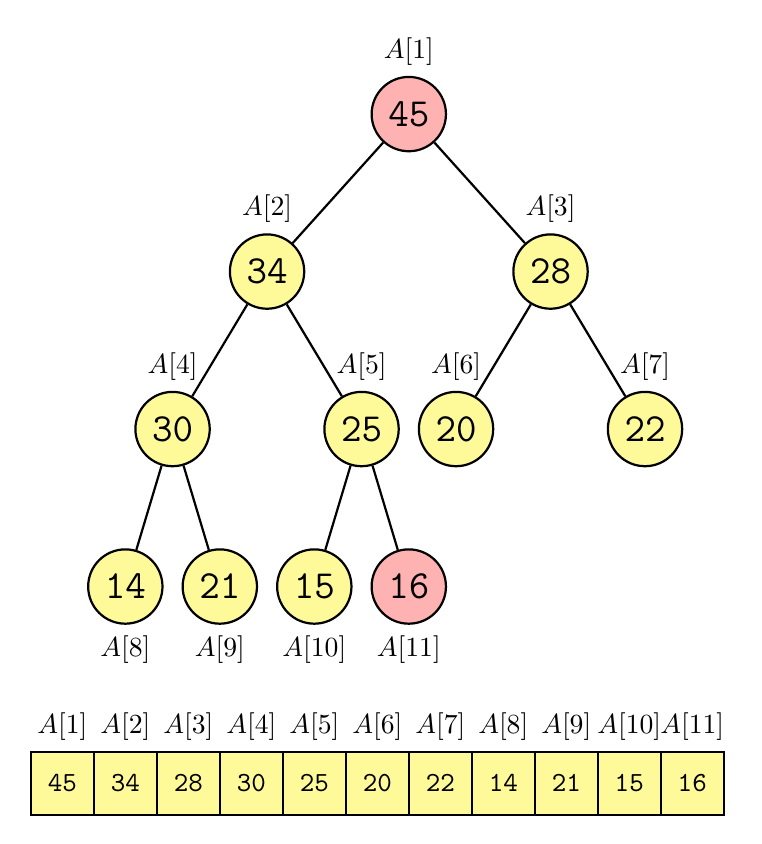
\begin{tikzpicture}[
  thick,
  level distance=2cm,
  level 1/.style={sibling distance=3.6cm},
  level 2/.style={sibling distance=2.4cm},
  level 3/.style={sibling distance=1.2cm},
	font=\ttfamily\bfseries]
  \node[mynoder, minimum size=0.9cm,label={above:$A[1]$}] at (0,0) {45}
    child {node[mynode, minimum size=0.9cm,label={above:$A[2]$}]  {34}
      child {node[mynode, minimum size=0.9cm,label={above:$A[4]$}] (a) {30}
        child {node[mynode, minimum size=0.9cm,label={below:$A[8]$}] (b) {14}}
        child {node[mynode, minimum size=0.9cm,label={below:$A[9]$}] {21}}
      }
      child {node[mynode, minimum size=0.9cm,label={above:$A[5]$}]  {25}
        child {node[mynode, minimum size=0.9cm,label={below:$A[10]$}] {15}}
        child {node[mynoder, minimum size=0.9cm,label={below:$A[11]$}] {16}}
      }
    }
    child {node[mynode, minimum size=0.9cm,label={above:$A[3]$}] {28}
      child {node[mynode, minimum size=0.9cm,label={above:$A[6]$}] {20}
      }
      child {node[mynode, minimum size=0.9cm,label={above:$A[7]$}] {22}
      }
    };
    
\node[draw,rectangle,minimum size=0.80cm,label={above:$A[1]$}, fill=yellow!40] at (-4.40,-8.5) {45};
\node[draw,rectangle,minimum size=0.80cm,label={above:$A[2]$}, fill=yellow!40] at (-3.60,-8.5) {34};
\node[draw,rectangle,minimum size=0.80cm,label={above:$A[3]$}, fill=yellow!40] at (-2.80,-8.5) {28};
\node[draw,rectangle,minimum size=0.80cm,label={above:$A[4]$}, fill=yellow!40] at (-2.00,-8.5) {30};
\node[draw,rectangle,minimum size=0.80cm,label={above:$A[5]$}, fill=yellow!40] at (-1.20,-8.5) {25};
\node[draw,rectangle,minimum size=0.80cm,label={above:$A[6]$}, fill=yellow!40] at (-0.40,-8.5) {20};
\node[draw,rectangle,minimum size=0.80cm,label={above:$A[7]$}, fill=yellow!40] at ( 0.40,-8.5) {22};
\node[draw,rectangle,minimum size=0.80cm,label={above:$A[8]$}, fill=yellow!40] at ( 1.20,-8.5) {14};
\node[draw,rectangle,minimum size=0.80cm,label={above:$A[9]$}, fill=yellow!40] at ( 2.00,-8.5) {21};
\node[draw,rectangle,minimum size=0.80cm,label={above:$A[10]$}, fill=yellow!40] at ( 2.80,-8.5) {15};
\node[draw,rectangle,minimum size=0.80cm,label={above:$A[11]$}, fill=yellow!40] at ( 3.60,-8.5) {16};
 \end{tikzpicture}

\newpage

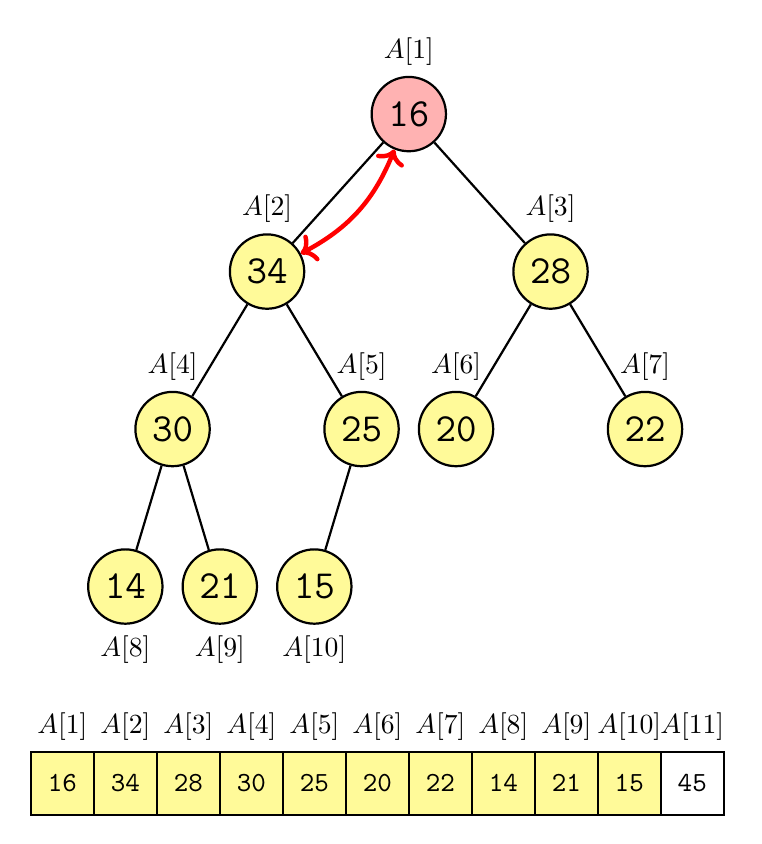
\begin{tikzpicture}[
  thick,
  level distance=2cm,
  level 1/.style={sibling distance=3.6cm},
  level 2/.style={sibling distance=2.4cm},
  level 3/.style={sibling distance=1.2cm},
	font=\ttfamily\bfseries]
  \node[mynoder, minimum size=0.9cm,label={above:$A[1]$}] at (0,0) (a) {16}
    child {node[mynode, minimum size=0.9cm,label={above:$A[2]$}]  (b) {34}
      child {node[mynode, minimum size=0.9cm,label={above:$A[4]$}]  {30}
        child {node[mynode, minimum size=0.9cm,label={below:$A[8]$}]  {14}}
        child {node[mynode, minimum size=0.9cm,label={below:$A[9]$}] {21}}
      }
      child {node[mynode, minimum size=0.9cm,label={above:$A[5]$}]  {25}
        child {node[mynode, minimum size=0.9cm,label={below:$A[10]$}] {15}}
        child[missing] {node[mynoder, minimum size=0.9cm,label={below:$A[11]$}] {16}}
      }
    }
    child {node[mynode, minimum size=0.9cm,label={above:$A[3]$}] {28}
      child {node[mynode, minimum size=0.9cm,label={above:$A[6]$}] {20}
      }
      child {node[mynode, minimum size=0.9cm,label={above:$A[7]$}] {22}
      }
    };
    
\node[draw,rectangle,minimum size=0.80cm,label={above:$A[1]$}, fill=yellow!40] at (-4.40,-8.5) {16};
\node[draw,rectangle,minimum size=0.80cm,label={above:$A[2]$}, fill=yellow!40] at (-3.60,-8.5) {34};
\node[draw,rectangle,minimum size=0.80cm,label={above:$A[3]$}, fill=yellow!40] at (-2.80,-8.5) {28};
\node[draw,rectangle,minimum size=0.80cm,label={above:$A[4]$}, fill=yellow!40] at (-2.00,-8.5) {30};
\node[draw,rectangle,minimum size=0.80cm,label={above:$A[5]$}, fill=yellow!40] at (-1.20,-8.5) {25};
\node[draw,rectangle,minimum size=0.80cm,label={above:$A[6]$}, fill=yellow!40] at (-0.40,-8.5) {20};
\node[draw,rectangle,minimum size=0.80cm,label={above:$A[7]$}, fill=yellow!40] at ( 0.40,-8.5) {22};
\node[draw,rectangle,minimum size=0.80cm,label={above:$A[8]$}, fill=yellow!40] at ( 1.20,-8.5) {14};
\node[draw,rectangle,minimum size=0.80cm,label={above:$A[9]$}, fill=yellow!40] at ( 2.00,-8.5) {21};
\node[draw,rectangle,minimum size=0.80cm,label={above:$A[10]$}, fill=yellow!40] at ( 2.80,-8.5) {15};
\node[draw,rectangle,minimum size=0.80cm,label={above:$A[11]$}] at ( 3.60,-8.5) {45};

  \draw[edger,<->] (a) edge[bend left=20] node {} (b);

 \end{tikzpicture}

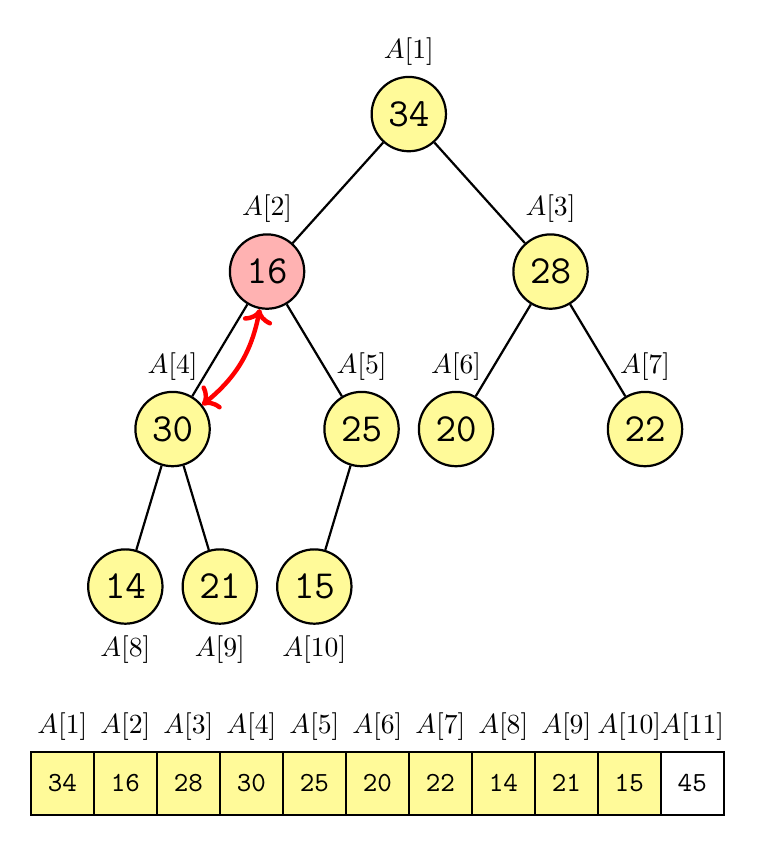
\begin{tikzpicture}[
  thick,
  level distance=2cm,
  level 1/.style={sibling distance=3.6cm},
  level 2/.style={sibling distance=2.4cm},
  level 3/.style={sibling distance=1.2cm},
	font=\ttfamily\bfseries]
  \node[mynode, minimum size=0.9cm,label={above:$A[1]$}] at (0,0) {34}
    child {node[mynoder, minimum size=0.9cm,label={above:$A[2]$}]  (a) {16}
      child {node[mynode, minimum size=0.9cm,label={above:$A[4]$}] (b) {30}
        child {node[mynode, minimum size=0.9cm,label={below:$A[8]$}]  {14}}
        child {node[mynode, minimum size=0.9cm,label={below:$A[9]$}] {21}}
      }
      child {node[mynode, minimum size=0.9cm,label={above:$A[5]$}]  {25}
        child {node[mynode, minimum size=0.9cm,label={below:$A[10]$}] {15}}
        child[missing] {node[mynoder, minimum size=0.9cm,label={below:$A[11]$}] {16}}
      }
    }
    child {node[mynode, minimum size=0.9cm,label={above:$A[3]$}] {28}
      child {node[mynode, minimum size=0.9cm,label={above:$A[6]$}] {20}
      }
      child {node[mynode, minimum size=0.9cm,label={above:$A[7]$}] {22}
      }
    };
    
\node[draw,rectangle,minimum size=0.80cm,label={above:$A[1]$}, fill=yellow!40] at (-4.40,-8.5) {34};
\node[draw,rectangle,minimum size=0.80cm,label={above:$A[2]$}, fill=yellow!40] at (-3.60,-8.5) {16};
\node[draw,rectangle,minimum size=0.80cm,label={above:$A[3]$}, fill=yellow!40] at (-2.80,-8.5) {28};
\node[draw,rectangle,minimum size=0.80cm,label={above:$A[4]$}, fill=yellow!40] at (-2.00,-8.5) {30};
\node[draw,rectangle,minimum size=0.80cm,label={above:$A[5]$}, fill=yellow!40] at (-1.20,-8.5) {25};
\node[draw,rectangle,minimum size=0.80cm,label={above:$A[6]$}, fill=yellow!40] at (-0.40,-8.5) {20};
\node[draw,rectangle,minimum size=0.80cm,label={above:$A[7]$}, fill=yellow!40] at ( 0.40,-8.5) {22};
\node[draw,rectangle,minimum size=0.80cm,label={above:$A[8]$}, fill=yellow!40] at ( 1.20,-8.5) {14};
\node[draw,rectangle,minimum size=0.80cm,label={above:$A[9]$}, fill=yellow!40] at ( 2.00,-8.5) {21};
\node[draw,rectangle,minimum size=0.80cm,label={above:$A[10]$}, fill=yellow!40] at ( 2.80,-8.5) {15};
\node[draw,rectangle,minimum size=0.80cm,label={above:$A[11]$}] at ( 3.60,-8.5) {45};

  \draw[edger,<->] (a) edge[bend left=20] node {} (b);

 \end{tikzpicture}

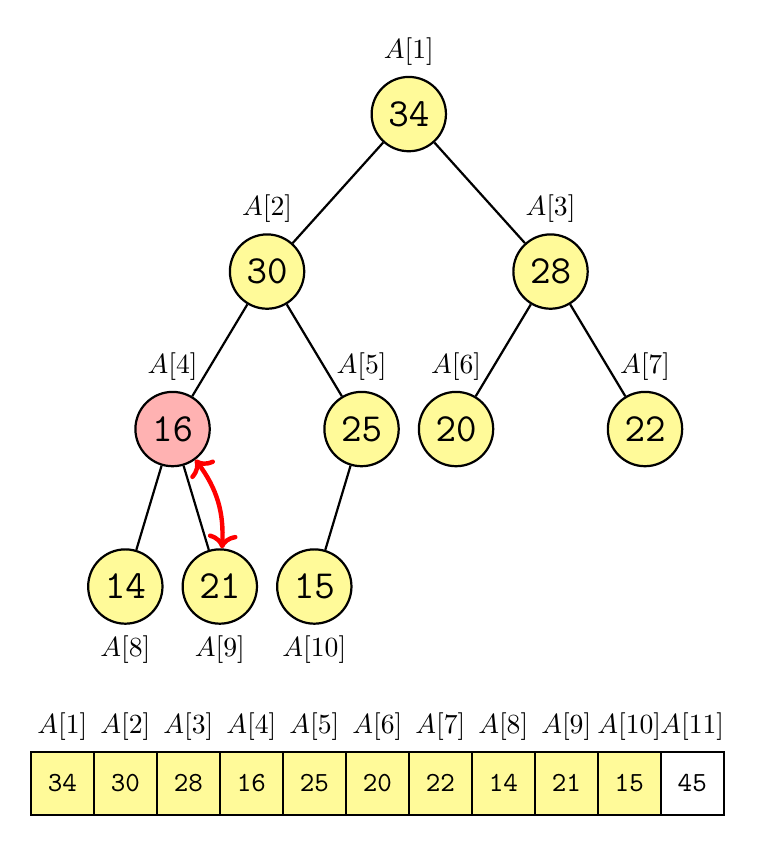
\begin{tikzpicture}[
  thick,
  level distance=2cm,
  level 1/.style={sibling distance=3.6cm},
  level 2/.style={sibling distance=2.4cm},
  level 3/.style={sibling distance=1.2cm},
	font=\ttfamily\bfseries]
  \node[mynode, minimum size=0.9cm,label={above:$A[1]$}] at (0,0) {34}
    child {node[mynode, minimum size=0.9cm,label={above:$A[2]$}]   {30}
      child {node[mynoder, minimum size=0.9cm,label={above:$A[4]$}] (a) {16}
        child {node[mynode, minimum size=0.9cm,label={below:$A[8]$}]  {14}}
        child {node[mynode, minimum size=0.9cm,label={below:$A[9]$}] (b) {21}}
      }
      child {node[mynode, minimum size=0.9cm,label={above:$A[5]$}]  {25}
        child {node[mynode, minimum size=0.9cm,label={below:$A[10]$}] {15}}
        child[missing] {node[mynoder, minimum size=0.9cm,label={below:$A[11]$}] {16}}
      }
    }
    child {node[mynode, minimum size=0.9cm,label={above:$A[3]$}] {28}
      child {node[mynode, minimum size=0.9cm,label={above:$A[6]$}] {20}
      }
      child {node[mynode, minimum size=0.9cm,label={above:$A[7]$}] {22}
      }
    };
    
\node[draw,rectangle,minimum size=0.80cm,label={above:$A[1]$}, fill=yellow!40] at (-4.40,-8.5) {34};
\node[draw,rectangle,minimum size=0.80cm,label={above:$A[2]$}, fill=yellow!40] at (-3.60,-8.5) {30};
\node[draw,rectangle,minimum size=0.80cm,label={above:$A[3]$}, fill=yellow!40] at (-2.80,-8.5) {28};
\node[draw,rectangle,minimum size=0.80cm,label={above:$A[4]$}, fill=yellow!40] at (-2.00,-8.5) {16};
\node[draw,rectangle,minimum size=0.80cm,label={above:$A[5]$}, fill=yellow!40] at (-1.20,-8.5) {25};
\node[draw,rectangle,minimum size=0.80cm,label={above:$A[6]$}, fill=yellow!40] at (-0.40,-8.5) {20};
\node[draw,rectangle,minimum size=0.80cm,label={above:$A[7]$}, fill=yellow!40] at ( 0.40,-8.5) {22};
\node[draw,rectangle,minimum size=0.80cm,label={above:$A[8]$}, fill=yellow!40] at ( 1.20,-8.5) {14};
\node[draw,rectangle,minimum size=0.80cm,label={above:$A[9]$}, fill=yellow!40] at ( 2.00,-8.5) {21};
\node[draw,rectangle,minimum size=0.80cm,label={above:$A[10]$}, fill=yellow!40] at ( 2.80,-8.5) {15};
\node[draw,rectangle,minimum size=0.80cm,label={above:$A[11]$}] at ( 3.60,-8.5) {45};

  \draw[edger,<->] (a) edge[bend left=20] node {} (b);

 \end{tikzpicture}

% \begin{tikzpicture}[
%   thick,
%   level distance=2cm,
%   level 1/.style={sibling distance=3.6cm},
%   level 2/.style={sibling distance=2.4cm},
%   level 3/.style={sibling distance=1.2cm},
%     font=\ttfamily\bfseries]
%   \node[mynode, minimum size=0.9cm,label={above:$A[1]$}] at (0,0) {34}
%     child {node[mynode, minimum size=0.9cm,label={above:$A[2]$}]   {30}
%       child {node[mynode, minimum size=0.9cm,label={above:$A[4]$}] (a) {21}
%         child {node[mynode, minimum size=0.9cm,label={below:$A[8]$}]  {14}}
%         child {node[mynoder, minimum size=0.9cm,label={below:$A[9]$}] (b) {16}}
%       }
%       child {node[mynode, minimum size=0.9cm,label={above:$A[5]$}]  {25}
%         child {node[mynode, minimum size=0.9cm,label={below:$A[10]$}] {15}}
%         child[missing] {node[mynoder, minimum size=0.9cm,label={below:$A[11]$}] {16}}
%       }
%     }
%     child {node[mynode, minimum size=0.9cm,label={above:$A[3]$}] {28}
%       child {node[mynode, minimum size=0.9cm,label={above:$A[6]$}] {20}
%       }
%       child {node[mynode, minimum size=0.9cm,label={above:$A[7]$}] {22}
%       }
%     };
%
% \node[draw,rectangle,minimum size=0.80cm,label={above:$A[1]$}, fill=yellow!40] at (-4.40,-8.5) {34};
% \node[draw,rectangle,minimum size=0.80cm,label={above:$A[2]$}, fill=yellow!40] at (-3.60,-8.5) {30};
% \node[draw,rectangle,minimum size=0.80cm,label={above:$A[3]$}, fill=yellow!40] at (-2.80,-8.5) {28};
% \node[draw,rectangle,minimum size=0.80cm,label={above:$A[4]$}, fill=yellow!40] at (-2.00,-8.5) {21};
% \node[draw,rectangle,minimum size=0.80cm,label={above:$A[5]$}, fill=yellow!40] at (-1.20,-8.5) {25};
% \node[draw,rectangle,minimum size=0.80cm,label={above:$A[6]$}, fill=yellow!40] at (-0.40,-8.5) {20};
% \node[draw,rectangle,minimum size=0.80cm,label={above:$A[7]$}, fill=yellow!40] at ( 0.40,-8.5) {22};
% \node[draw,rectangle,minimum size=0.80cm,label={above:$A[8]$}, fill=yellow!40] at ( 1.20,-8.5) {14};
% \node[draw,rectangle,minimum size=0.80cm,label={above:$A[9]$}, fill=yellow!40] at ( 2.00,-8.5) {16};
% \node[draw,rectangle,minimum size=0.80cm,label={above:$A[10]$}, fill=yellow!40] at ( 2.80,-8.5) {15};
% \node[draw,rectangle,minimum size=0.80cm,label={above:$A[11]$}] at ( 3.60,-8.5) {45};
%
%
%  \end{tikzpicture}

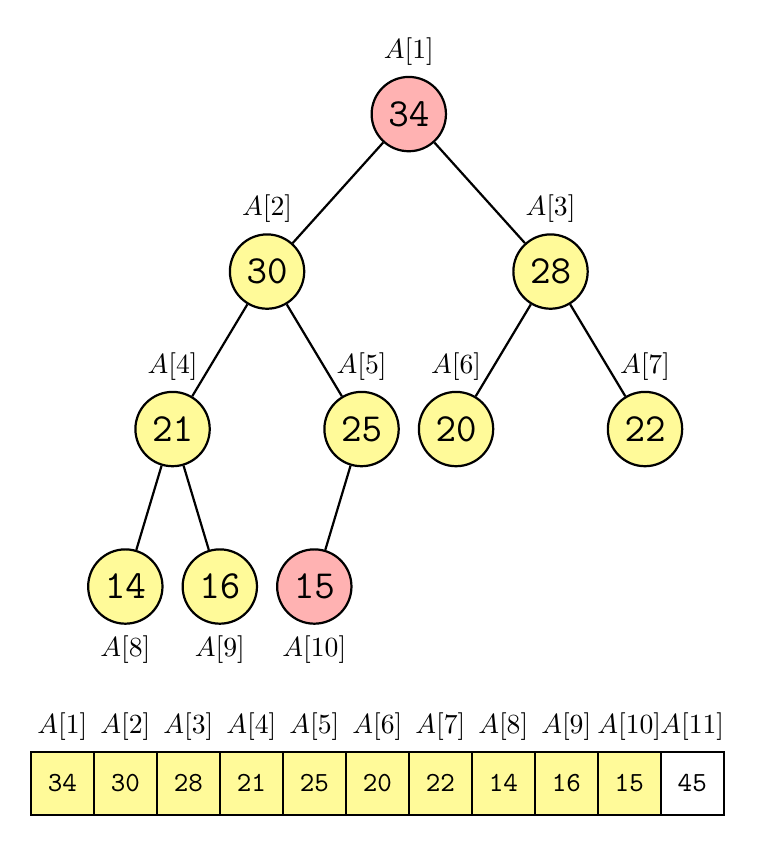
\begin{tikzpicture}[
  thick,
  level distance=2cm,
  level 1/.style={sibling distance=3.6cm},
  level 2/.style={sibling distance=2.4cm},
  level 3/.style={sibling distance=1.2cm},
	font=\ttfamily\bfseries]
  \node[mynoder, minimum size=0.9cm,label={above:$A[1]$}] at (0,0) {34}
    child {node[mynode, minimum size=0.9cm,label={above:$A[2]$}]   {30}
      child {node[mynode, minimum size=0.9cm,label={above:$A[4]$}] (a) {21}
        child {node[mynode, minimum size=0.9cm,label={below:$A[8]$}]  {14}}
        child {node[mynode, minimum size=0.9cm,label={below:$A[9]$}] (b) {16}}
      }
      child {node[mynode, minimum size=0.9cm,label={above:$A[5]$}]  {25}
        child {node[mynoder, minimum size=0.9cm,label={below:$A[10]$}] {15}}
        child[missing] {node[mynoder, minimum size=0.9cm,label={below:$A[11]$}] {16}}
      }
    }
    child {node[mynode, minimum size=0.9cm,label={above:$A[3]$}] {28}
      child {node[mynode, minimum size=0.9cm,label={above:$A[6]$}] {20}
      }
      child {node[mynode, minimum size=0.9cm,label={above:$A[7]$}] {22}
      }
    };
    
\node[draw,rectangle,minimum size=0.80cm,label={above:$A[1]$}, fill=yellow!40] at (-4.40,-8.5) {34};
\node[draw,rectangle,minimum size=0.80cm,label={above:$A[2]$}, fill=yellow!40] at (-3.60,-8.5) {30};
\node[draw,rectangle,minimum size=0.80cm,label={above:$A[3]$}, fill=yellow!40] at (-2.80,-8.5) {28};
\node[draw,rectangle,minimum size=0.80cm,label={above:$A[4]$}, fill=yellow!40] at (-2.00,-8.5) {21};
\node[draw,rectangle,minimum size=0.80cm,label={above:$A[5]$}, fill=yellow!40] at (-1.20,-8.5) {25};
\node[draw,rectangle,minimum size=0.80cm,label={above:$A[6]$}, fill=yellow!40] at (-0.40,-8.5) {20};
\node[draw,rectangle,minimum size=0.80cm,label={above:$A[7]$}, fill=yellow!40] at ( 0.40,-8.5) {22};
\node[draw,rectangle,minimum size=0.80cm,label={above:$A[8]$}, fill=yellow!40] at ( 1.20,-8.5) {14};
\node[draw,rectangle,minimum size=0.80cm,label={above:$A[9]$}, fill=yellow!40] at ( 2.00,-8.5) {16};
\node[draw,rectangle,minimum size=0.80cm,label={above:$A[10]$}, fill=yellow!40] at ( 2.80,-8.5) {15};
\node[draw,rectangle,minimum size=0.80cm,label={above:$A[11]$}] at ( 3.60,-8.5) {45};


 \end{tikzpicture}

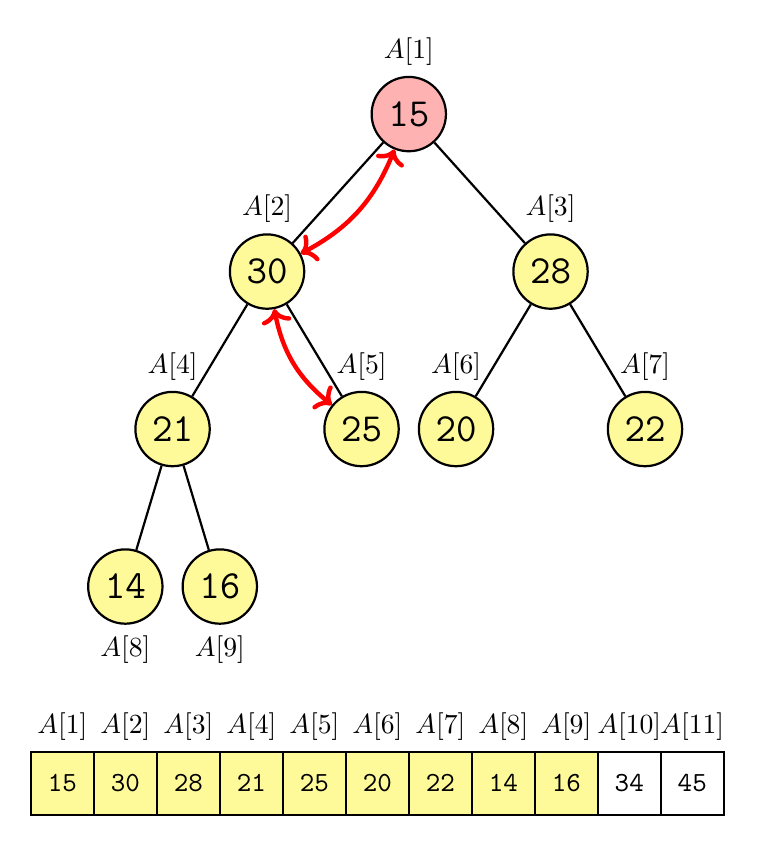
\begin{tikzpicture}[
  thick,
  level distance=2cm,
  level 1/.style={sibling distance=3.6cm},
  level 2/.style={sibling distance=2.4cm},
  level 3/.style={sibling distance=1.2cm},
	font=\ttfamily\bfseries]
  \node[mynoder, minimum size=0.9cm,label={above:$A[1]$}] at (0,0) (a) {15}
    child {node[mynode, minimum size=0.9cm,label={above:$A[2]$}] (b)  {30}
      child {node[mynode, minimum size=0.9cm,label={above:$A[4]$}]  {21}
        child {node[mynode, minimum size=0.9cm,label={below:$A[8]$}]  {14}}
        child {node[mynode, minimum size=0.9cm,label={below:$A[9]$}]  {16}}
      }
      child {node[mynode, minimum size=0.9cm,label={above:$A[5]$}] (c) {25}
        child[missing] {node[mynoder, minimum size=0.9cm,label={below:$A[10]$}] {15}}
        child[missing] {node[mynoder, minimum size=0.9cm,label={below:$A[11]$}] {16}}
      }
    }
    child {node[mynode, minimum size=0.9cm,label={above:$A[3]$}] {28}
      child {node[mynode, minimum size=0.9cm,label={above:$A[6]$}] {20}
      }
      child {node[mynode, minimum size=0.9cm,label={above:$A[7]$}] {22}
      }
    };
    
\node[draw,rectangle,minimum size=0.80cm,label={above:$A[1]$}, fill=yellow!40] at (-4.40,-8.5) {15};
\node[draw,rectangle,minimum size=0.80cm,label={above:$A[2]$}, fill=yellow!40] at (-3.60,-8.5) {30};
\node[draw,rectangle,minimum size=0.80cm,label={above:$A[3]$}, fill=yellow!40] at (-2.80,-8.5) {28};
\node[draw,rectangle,minimum size=0.80cm,label={above:$A[4]$}, fill=yellow!40] at (-2.00,-8.5) {21};
\node[draw,rectangle,minimum size=0.80cm,label={above:$A[5]$}, fill=yellow!40] at (-1.20,-8.5) {25};
\node[draw,rectangle,minimum size=0.80cm,label={above:$A[6]$}, fill=yellow!40] at (-0.40,-8.5) {20};
\node[draw,rectangle,minimum size=0.80cm,label={above:$A[7]$}, fill=yellow!40] at ( 0.40,-8.5) {22};
\node[draw,rectangle,minimum size=0.80cm,label={above:$A[8]$}, fill=yellow!40] at ( 1.20,-8.5) {14};
\node[draw,rectangle,minimum size=0.80cm,label={above:$A[9]$}, fill=yellow!40] at ( 2.00,-8.5) {16};
\node[draw,rectangle,minimum size=0.80cm,label={above:$A[10]$}] at ( 2.80,-8.5) {34};
\node[draw,rectangle,minimum size=0.80cm,label={above:$A[11]$}] at ( 3.60,-8.5) {45};

  \draw[edger,<->] (a) edge[bend left=20] node {} (b);
  \draw[edger,<->] (b) edge[bend right=20] node {} (c);

 \end{tikzpicture}


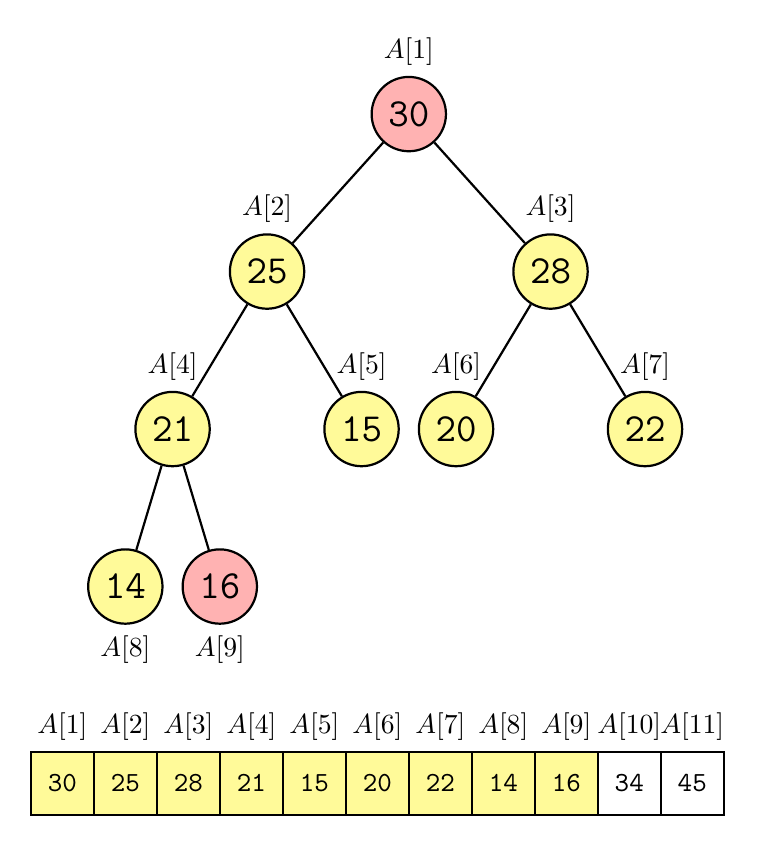
\begin{tikzpicture}[
  thick,
  level distance=2cm,
  level 1/.style={sibling distance=3.6cm},
  level 2/.style={sibling distance=2.4cm},
  level 3/.style={sibling distance=1.2cm},
	font=\ttfamily\bfseries]
  \node[mynoder, minimum size=0.9cm,label={above:$A[1]$}] at (0,0)  {30}
    child {node[mynode, minimum size=0.9cm,label={above:$A[2]$}] (a)  {25}
      child {node[mynode, minimum size=0.9cm,label={above:$A[4]$}]  {21}
        child {node[mynode, minimum size=0.9cm,label={below:$A[8]$}]  {14}}
        child {node[mynoder, minimum size=0.9cm,label={below:$A[9]$}]  {16}}
      }
      child {node[mynode, minimum size=0.9cm,label={above:$A[5]$}] (b)  {15}
      }
    }
    child {node[mynode, minimum size=0.9cm,label={above:$A[3]$}] {28}
      child {node[mynode, minimum size=0.9cm,label={above:$A[6]$}] {20}
      }
      child {node[mynode, minimum size=0.9cm,label={above:$A[7]$}] {22}
      }
    };
    
\node[draw,rectangle,minimum size=0.80cm,label={above:$A[1]$}, fill=yellow!40] at (-4.40,-8.5) {30};
\node[draw,rectangle,minimum size=0.80cm,label={above:$A[2]$}, fill=yellow!40] at (-3.60,-8.5) {25};
\node[draw,rectangle,minimum size=0.80cm,label={above:$A[3]$}, fill=yellow!40] at (-2.80,-8.5) {28};
\node[draw,rectangle,minimum size=0.80cm,label={above:$A[4]$}, fill=yellow!40] at (-2.00,-8.5) {21};
\node[draw,rectangle,minimum size=0.80cm,label={above:$A[5]$}, fill=yellow!40] at (-1.20,-8.5) {15};
\node[draw,rectangle,minimum size=0.80cm,label={above:$A[6]$}, fill=yellow!40] at (-0.40,-8.5) {20};
\node[draw,rectangle,minimum size=0.80cm,label={above:$A[7]$}, fill=yellow!40] at ( 0.40,-8.5) {22};
\node[draw,rectangle,minimum size=0.80cm,label={above:$A[8]$}, fill=yellow!40] at ( 1.20,-8.5) {14};
\node[draw,rectangle,minimum size=0.80cm,label={above:$A[9]$}, fill=yellow!40] at ( 2.00,-8.5) {16};
\node[draw,rectangle,minimum size=0.80cm,label={above:$A[10]$}] at ( 2.80,-8.5) {34};
\node[draw,rectangle,minimum size=0.80cm,label={above:$A[11]$}] at ( 3.60,-8.5) {45};


 \end{tikzpicture}

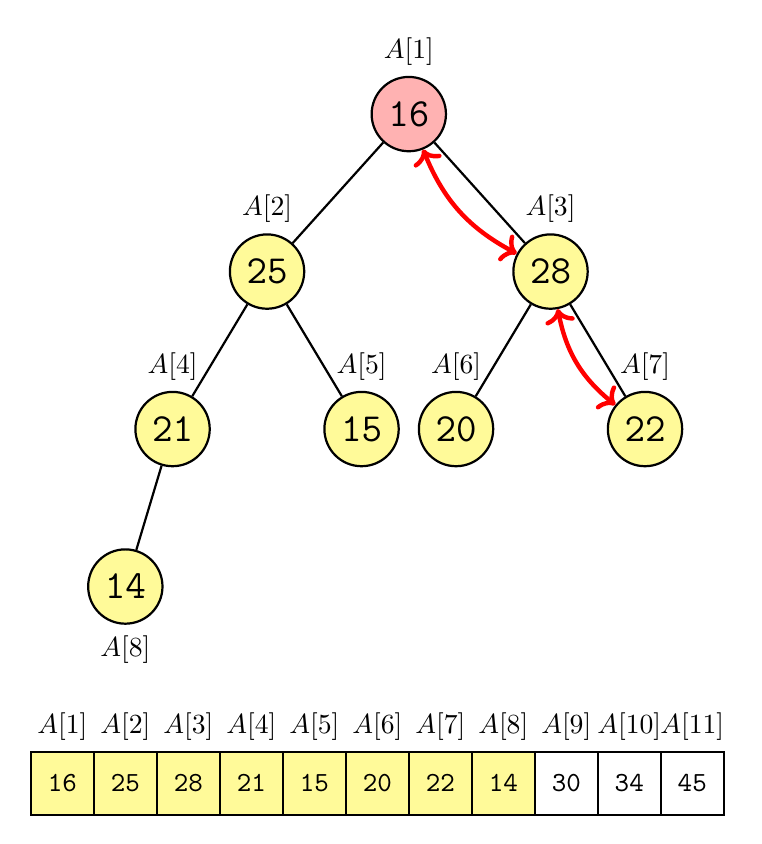
\begin{tikzpicture}[
  thick,
  level distance=2cm,
  level 1/.style={sibling distance=3.6cm},
  level 2/.style={sibling distance=2.4cm},
  level 3/.style={sibling distance=1.2cm},
	font=\ttfamily\bfseries]
  \node[mynoder, minimum size=0.9cm,label={above:$A[1]$}] at (0,0) (a) {16}
    child {node[mynode, minimum size=0.9cm,label={above:$A[2]$}]   {25}
      child {node[mynode, minimum size=0.9cm,label={above:$A[4]$}]  {21}
        child {node[mynode, minimum size=0.9cm,label={below:$A[8]$}]  {14}}
        child[missing] {node[mynode, minimum size=0.9cm,label={below:$A[9]$}]  {}}
      }
      child {node[mynode, minimum size=0.9cm,label={above:$A[5]$}]   {15}
      }
    }
    child {node[mynode, minimum size=0.9cm,label={above:$A[3]$}] (b) {28}
      child {node[mynode, minimum size=0.9cm,label={above:$A[6]$}] {20}
      }
      child {node[mynode, minimum size=0.9cm,label={above:$A[7]$}] (c) {22}
      }
    };
    
\node[draw,rectangle,minimum size=0.80cm,label={above:$A[1]$}, fill=yellow!40] at (-4.40,-8.5) {16};
\node[draw,rectangle,minimum size=0.80cm,label={above:$A[2]$}, fill=yellow!40] at (-3.60,-8.5) {25};
\node[draw,rectangle,minimum size=0.80cm,label={above:$A[3]$}, fill=yellow!40] at (-2.80,-8.5) {28};
\node[draw,rectangle,minimum size=0.80cm,label={above:$A[4]$}, fill=yellow!40] at (-2.00,-8.5) {21};
\node[draw,rectangle,minimum size=0.80cm,label={above:$A[5]$}, fill=yellow!40] at (-1.20,-8.5) {15};
\node[draw,rectangle,minimum size=0.80cm,label={above:$A[6]$}, fill=yellow!40] at (-0.40,-8.5) {20};
\node[draw,rectangle,minimum size=0.80cm,label={above:$A[7]$}, fill=yellow!40] at ( 0.40,-8.5) {22};
\node[draw,rectangle,minimum size=0.80cm,label={above:$A[8]$}, fill=yellow!40] at ( 1.20,-8.5) {14};
\node[draw,rectangle,minimum size=0.80cm,label={above:$A[9]$}] at ( 2.00,-8.5) {30};
\node[draw,rectangle,minimum size=0.80cm,label={above:$A[10]$}] at ( 2.80,-8.5) {34};
\node[draw,rectangle,minimum size=0.80cm,label={above:$A[11]$}] at ( 3.60,-8.5) {45};

  \draw[edger,<->] (a) edge[bend right=20] node {} (b);
  \draw[edger,<->] (b) edge[bend right=20] node {} (c);

 \end{tikzpicture}


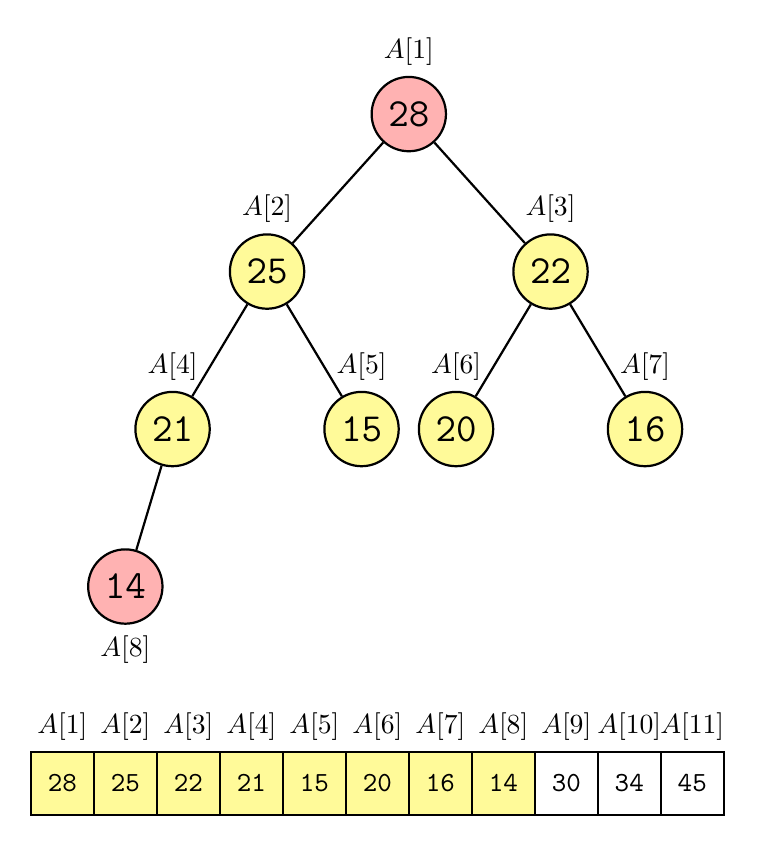
\begin{tikzpicture}[
  thick,
  level distance=2cm,
  level 1/.style={sibling distance=3.6cm},
  level 2/.style={sibling distance=2.4cm},
  level 3/.style={sibling distance=1.2cm},
	font=\ttfamily\bfseries]
  \node[mynoder, minimum size=0.9cm,label={above:$A[1]$}] at (0,0)  {28}
    child {node[mynode, minimum size=0.9cm,label={above:$A[2]$}]   {25}
      child {node[mynode, minimum size=0.9cm,label={above:$A[4]$}]  {21}
        child {node[mynoder, minimum size=0.9cm,label={below:$A[8]$}]  {14}}
        child[missing] {node[mynode, minimum size=0.9cm,label={below:$A[9]$}]  {}}
      }
      child {node[mynode, minimum size=0.9cm,label={above:$A[5]$}]   {15}
      }
    }
    child {node[mynode, minimum size=0.9cm,label={above:$A[3]$}] (a) {22}
      child {node[mynode, minimum size=0.9cm,label={above:$A[6]$}] {20}
      }
      child {node[mynode, minimum size=0.9cm,label={above:$A[7]$}] {16}
      }
    };
    
\node[draw,rectangle,minimum size=0.80cm,label={above:$A[1]$}, fill=yellow!40] at (-4.40,-8.5) {28};
\node[draw,rectangle,minimum size=0.80cm,label={above:$A[2]$}, fill=yellow!40] at (-3.60,-8.5) {25};
\node[draw,rectangle,minimum size=0.80cm,label={above:$A[3]$}, fill=yellow!40] at (-2.80,-8.5) {22};
\node[draw,rectangle,minimum size=0.80cm,label={above:$A[4]$}, fill=yellow!40] at (-2.00,-8.5) {21};
\node[draw,rectangle,minimum size=0.80cm,label={above:$A[5]$}, fill=yellow!40] at (-1.20,-8.5) {15};
\node[draw,rectangle,minimum size=0.80cm,label={above:$A[6]$}, fill=yellow!40] at (-0.40,-8.5) {20};
\node[draw,rectangle,minimum size=0.80cm,label={above:$A[7]$}, fill=yellow!40] at ( 0.40,-8.5) {16};
\node[draw,rectangle,minimum size=0.80cm,label={above:$A[8]$}, fill=yellow!40] at ( 1.20,-8.5) {14};
\node[draw,rectangle,minimum size=0.80cm,label={above:$A[9]$}] at ( 2.00,-8.5) {30};
\node[draw,rectangle,minimum size=0.80cm,label={above:$A[10]$}] at ( 2.80,-8.5) {34};
\node[draw,rectangle,minimum size=0.80cm,label={above:$A[11]$}] at ( 3.60,-8.5) {45};


 \end{tikzpicture}

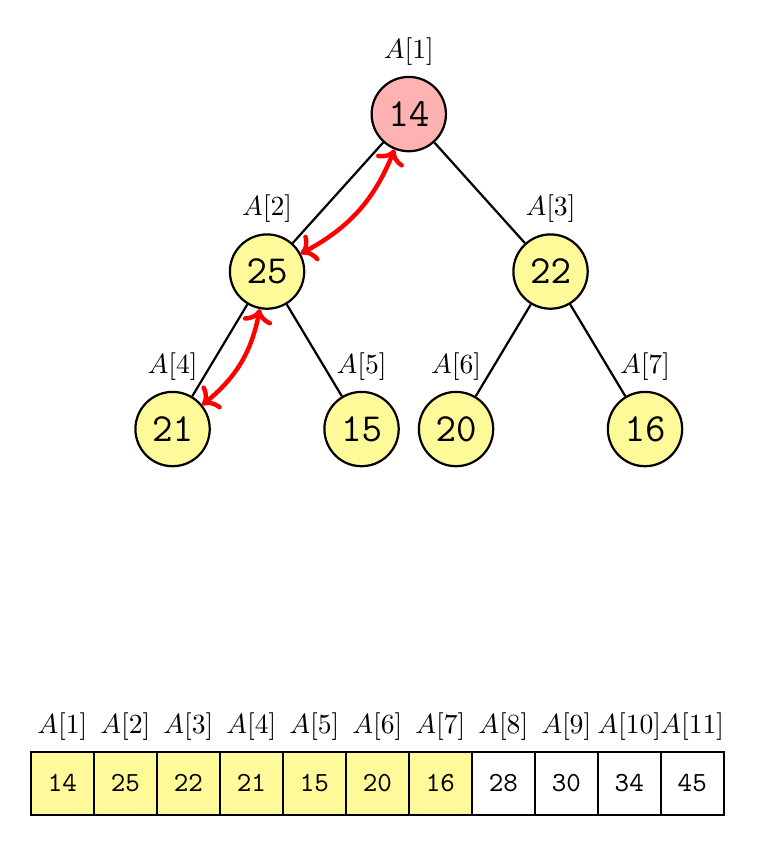
\begin{tikzpicture}[
  thick,
  level distance=2cm,
  level 1/.style={sibling distance=3.6cm},
  level 2/.style={sibling distance=2.4cm},
  level 3/.style={sibling distance=1.2cm},
	font=\ttfamily\bfseries]
  \node[mynoder, minimum size=0.9cm,label={above:$A[1]$}] at (0,0) (a) {14}
    child {node[mynode, minimum size=0.9cm,label={above:$A[2]$}] (b)  {25}
      child {node[mynode, minimum size=0.9cm,label={above:$A[4]$}] (c) {21}}
      child {node[mynode, minimum size=0.9cm,label={above:$A[5]$}]    {15}}
    }
    child {node[mynode, minimum size=0.9cm,label={above:$A[3]$}]  {22}
      child {node[mynode, minimum size=0.9cm,label={above:$A[6]$}] {20}}
      child {node[mynode, minimum size=0.9cm,label={above:$A[7]$}] {16}}
    };
    
\node[draw,rectangle,minimum size=0.80cm,label={above:$A[1]$}, fill=yellow!40] at (-4.40,-8.5) {14};
\node[draw,rectangle,minimum size=0.80cm,label={above:$A[2]$}, fill=yellow!40] at (-3.60,-8.5) {25};
\node[draw,rectangle,minimum size=0.80cm,label={above:$A[3]$}, fill=yellow!40] at (-2.80,-8.5) {22};
\node[draw,rectangle,minimum size=0.80cm,label={above:$A[4]$}, fill=yellow!40] at (-2.00,-8.5) {21};
\node[draw,rectangle,minimum size=0.80cm,label={above:$A[5]$}, fill=yellow!40] at (-1.20,-8.5) {15};
\node[draw,rectangle,minimum size=0.80cm,label={above:$A[6]$}, fill=yellow!40] at (-0.40,-8.5) {20};
\node[draw,rectangle,minimum size=0.80cm,label={above:$A[7]$}, fill=yellow!40] at ( 0.40,-8.5) {16};
\node[draw,rectangle,minimum size=0.80cm,label={above:$A[8]$}] at ( 1.20,-8.5) {28};
\node[draw,rectangle,minimum size=0.80cm,label={above:$A[9]$}] at ( 2.00,-8.5) {30};
\node[draw,rectangle,minimum size=0.80cm,label={above:$A[10]$}] at ( 2.80,-8.5) {34};
\node[draw,rectangle,minimum size=0.80cm,label={above:$A[11]$}] at ( 3.60,-8.5) {45};

  \draw[edger,<->] (a) edge[bend left=20] node {} (b);
  \draw[edger,<->] (b) edge[bend left=20] node {} (c);

 \end{tikzpicture}

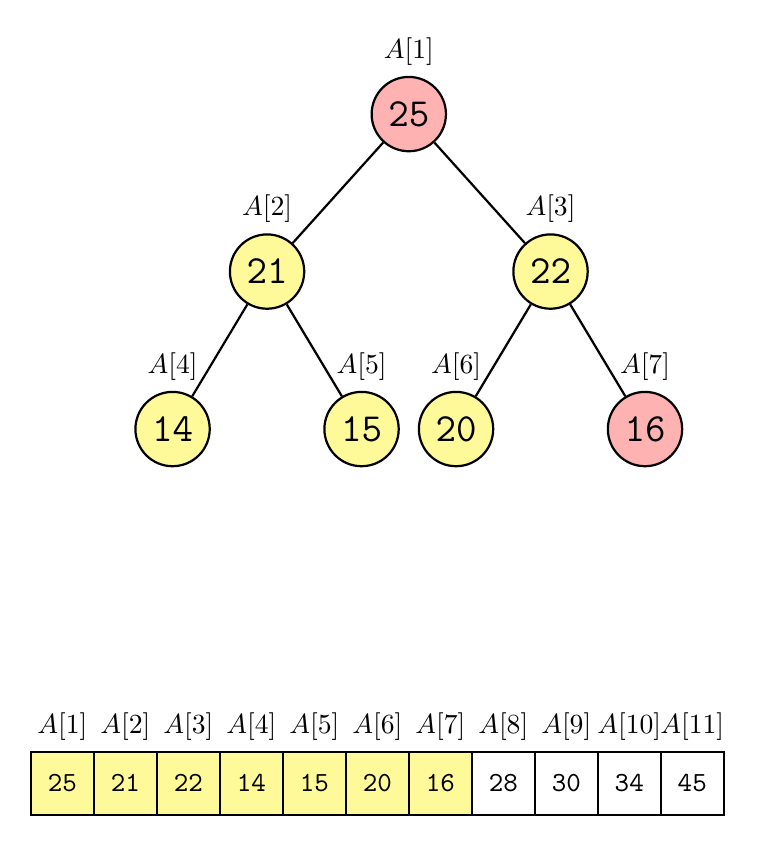
\begin{tikzpicture}[
  thick,
  level distance=2cm,
  level 1/.style={sibling distance=3.6cm},
  level 2/.style={sibling distance=2.4cm},
  level 3/.style={sibling distance=1.2cm},
	font=\ttfamily\bfseries]
  \node[mynoder, minimum size=0.9cm,label={above:$A[1]$}] at (0,0) (a) {25}
    child {node[mynode, minimum size=0.9cm,label={above:$A[2]$}]   {21}
      child {node[mynode, minimum size=0.9cm,label={above:$A[4]$}]  {14}}
      child {node[mynode, minimum size=0.9cm,label={above:$A[5]$}] (c)   {15}}
    }
    child {node[mynode, minimum size=0.9cm,label={above:$A[3]$}]  {22}
      child {node[mynode, minimum size=0.9cm,label={above:$A[6]$}] {20}}
      child {node[mynoder, minimum size=0.9cm,label={above:$A[7]$}] {16}}
    };
    
\node[draw,rectangle,minimum size=0.80cm,label={above:$A[1]$}, fill=yellow!40] at (-4.40,-8.5) {25};
\node[draw,rectangle,minimum size=0.80cm,label={above:$A[2]$}, fill=yellow!40] at (-3.60,-8.5) {21};
\node[draw,rectangle,minimum size=0.80cm,label={above:$A[3]$}, fill=yellow!40] at (-2.80,-8.5) {22};
\node[draw,rectangle,minimum size=0.80cm,label={above:$A[4]$}, fill=yellow!40] at (-2.00,-8.5) {14};
\node[draw,rectangle,minimum size=0.80cm,label={above:$A[5]$}, fill=yellow!40] at (-1.20,-8.5) {15};
\node[draw,rectangle,minimum size=0.80cm,label={above:$A[6]$}, fill=yellow!40] at (-0.40,-8.5) {20};
\node[draw,rectangle,minimum size=0.80cm,label={above:$A[7]$}, fill=yellow!40] at ( 0.40,-8.5) {16};
\node[draw,rectangle,minimum size=0.80cm,label={above:$A[8]$}] at ( 1.20,-8.5) {28};
\node[draw,rectangle,minimum size=0.80cm,label={above:$A[9]$}] at ( 2.00,-8.5) {30};
\node[draw,rectangle,minimum size=0.80cm,label={above:$A[10]$}] at ( 2.80,-8.5) {34};
\node[draw,rectangle,minimum size=0.80cm,label={above:$A[11]$}] at ( 3.60,-8.5) {45};


 \end{tikzpicture}

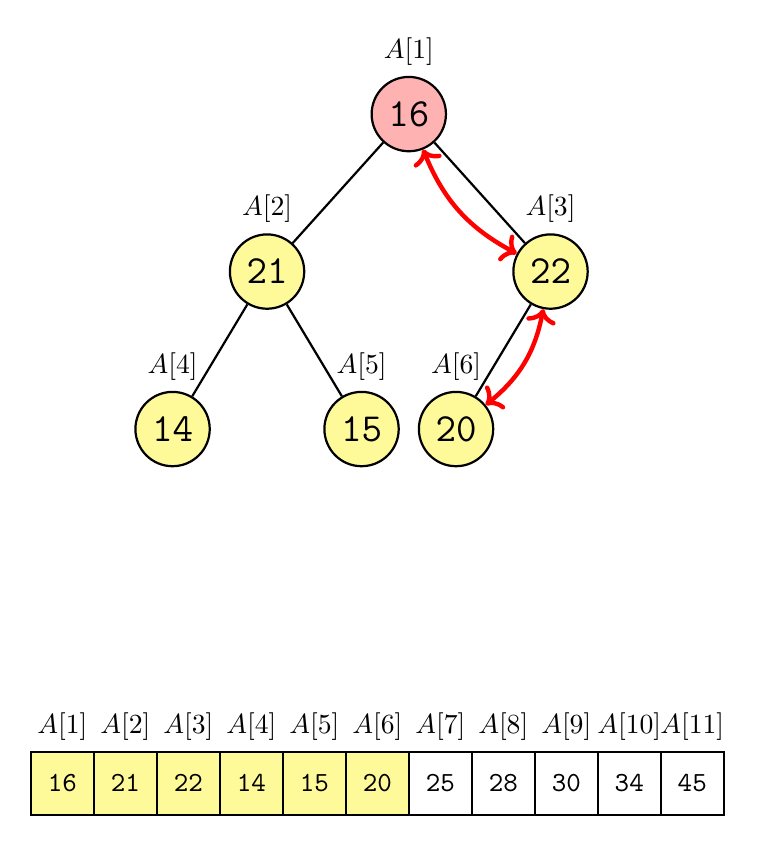
\begin{tikzpicture}[
  thick,
  level distance=2cm,
  level 1/.style={sibling distance=3.6cm},
  level 2/.style={sibling distance=2.4cm},
  level 3/.style={sibling distance=1.2cm},
	font=\ttfamily\bfseries]
  \node[mynoder, minimum size=0.9cm,label={above:$A[1]$}] at (0,0) (a) {16}
    child {node[mynode, minimum size=0.9cm,label={above:$A[2]$}]   {21}
      child {node[mynode, minimum size=0.9cm,label={above:$A[4]$}] {14}}
      child {node[mynode, minimum size=0.9cm,label={above:$A[5]$}] (c)   {15}}
    }
    child {node[mynode, minimum size=0.9cm,label={above:$A[3]$}] (b) {22}
      child {node[mynode, minimum size=0.9cm,label={above:$A[6]$}] (c) {20}}
      child[missing] {node[mynoder, minimum size=0.9cm,label={above:$A[7]$}] {16}}
    };
    
\node[draw,rectangle,minimum size=0.80cm,label={above:$A[1]$}, fill=yellow!40] at (-4.40,-8.5) {16};
\node[draw,rectangle,minimum size=0.80cm,label={above:$A[2]$}, fill=yellow!40] at (-3.60,-8.5) {21};
\node[draw,rectangle,minimum size=0.80cm,label={above:$A[3]$}, fill=yellow!40] at (-2.80,-8.5) {22};
\node[draw,rectangle,minimum size=0.80cm,label={above:$A[4]$}, fill=yellow!40] at (-2.00,-8.5) {14};
\node[draw,rectangle,minimum size=0.80cm,label={above:$A[5]$}, fill=yellow!40] at (-1.20,-8.5) {15};
\node[draw,rectangle,minimum size=0.80cm,label={above:$A[6]$}, fill=yellow!40] at (-0.40,-8.5) {20};
\node[draw,rectangle,minimum size=0.80cm,label={above:$A[7]$}] at ( 0.40,-8.5) {25};
\node[draw,rectangle,minimum size=0.80cm,label={above:$A[8]$}] at ( 1.20,-8.5) {28};
\node[draw,rectangle,minimum size=0.80cm,label={above:$A[9]$}] at ( 2.00,-8.5) {30};
\node[draw,rectangle,minimum size=0.80cm,label={above:$A[10]$}] at ( 2.80,-8.5) {34};
\node[draw,rectangle,minimum size=0.80cm,label={above:$A[11]$}] at ( 3.60,-8.5) {45};

  \draw[edger,<->] (a) edge[bend right=20] node {} (b);
  \draw[edger,<->] (b) edge[bend left=20] node {} (c);

 \end{tikzpicture}

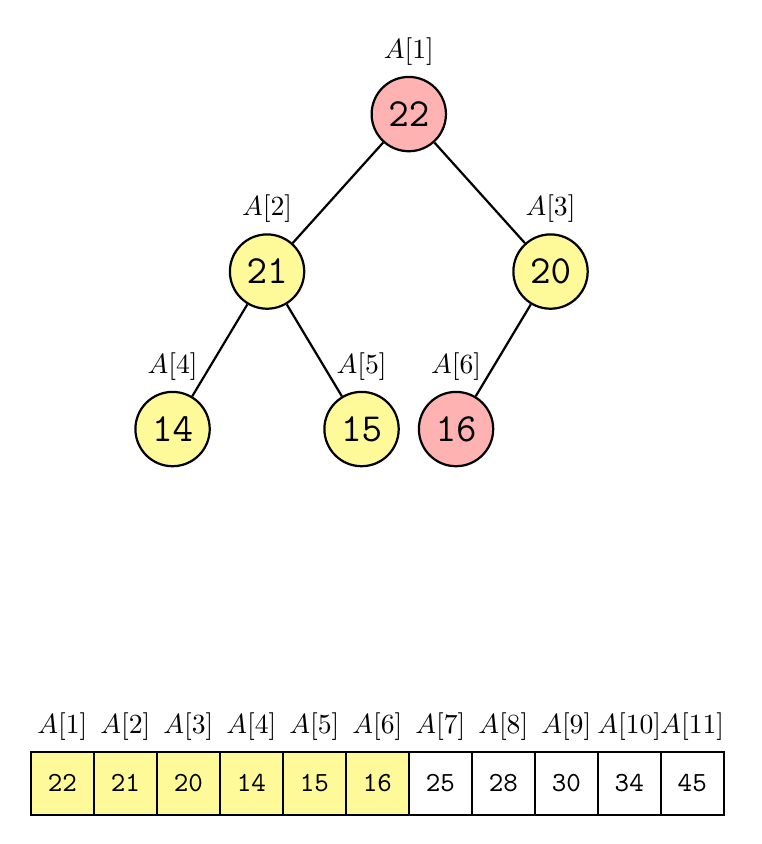
\begin{tikzpicture}[
  thick,
  level distance=2cm,
  level 1/.style={sibling distance=3.6cm},
  level 2/.style={sibling distance=2.4cm},
  level 3/.style={sibling distance=1.2cm},
	font=\ttfamily\bfseries]
  \node[mynoder, minimum size=0.9cm,label={above:$A[1]$}] at (0,0) (a) {22}
    child {node[mynode, minimum size=0.9cm,label={above:$A[2]$}]   {21}
      child {node[mynode, minimum size=0.9cm,label={above:$A[4]$}] {14}}
      child {node[mynode, minimum size=0.9cm,label={above:$A[5]$}] (c)   {15}}
    }
    child {node[mynode, minimum size=0.9cm,label={above:$A[3]$}] (b) {20}
      child {node[mynoder, minimum size=0.9cm,label={above:$A[6]$}] (c) {16}}
      child[missing] {node[mynoder, minimum size=0.9cm,label={above:$A[7]$}] {16}}
    };
    
\node[draw,rectangle,minimum size=0.80cm,label={above:$A[1]$}, fill=yellow!40] at (-4.40,-8.5) {22};
\node[draw,rectangle,minimum size=0.80cm,label={above:$A[2]$}, fill=yellow!40] at (-3.60,-8.5) {21};
\node[draw,rectangle,minimum size=0.80cm,label={above:$A[3]$}, fill=yellow!40] at (-2.80,-8.5) {20};
\node[draw,rectangle,minimum size=0.80cm,label={above:$A[4]$}, fill=yellow!40] at (-2.00,-8.5) {14};
\node[draw,rectangle,minimum size=0.80cm,label={above:$A[5]$}, fill=yellow!40] at (-1.20,-8.5) {15};
\node[draw,rectangle,minimum size=0.80cm,label={above:$A[6]$}, fill=yellow!40] at (-0.40,-8.5) {16};
\node[draw,rectangle,minimum size=0.80cm,label={above:$A[7]$}] at ( 0.40,-8.5) {25};
\node[draw,rectangle,minimum size=0.80cm,label={above:$A[8]$}] at ( 1.20,-8.5) {28};
\node[draw,rectangle,minimum size=0.80cm,label={above:$A[9]$}] at ( 2.00,-8.5) {30};
\node[draw,rectangle,minimum size=0.80cm,label={above:$A[10]$}] at ( 2.80,-8.5) {34};
\node[draw,rectangle,minimum size=0.80cm,label={above:$A[11]$}] at ( 3.60,-8.5) {45};

  % \draw[edger,<->] (a) edge[bend right=20] node {} (b);
  % \draw[edger,<->] (b) edge[bend left=20] node {} (c);

 \end{tikzpicture}

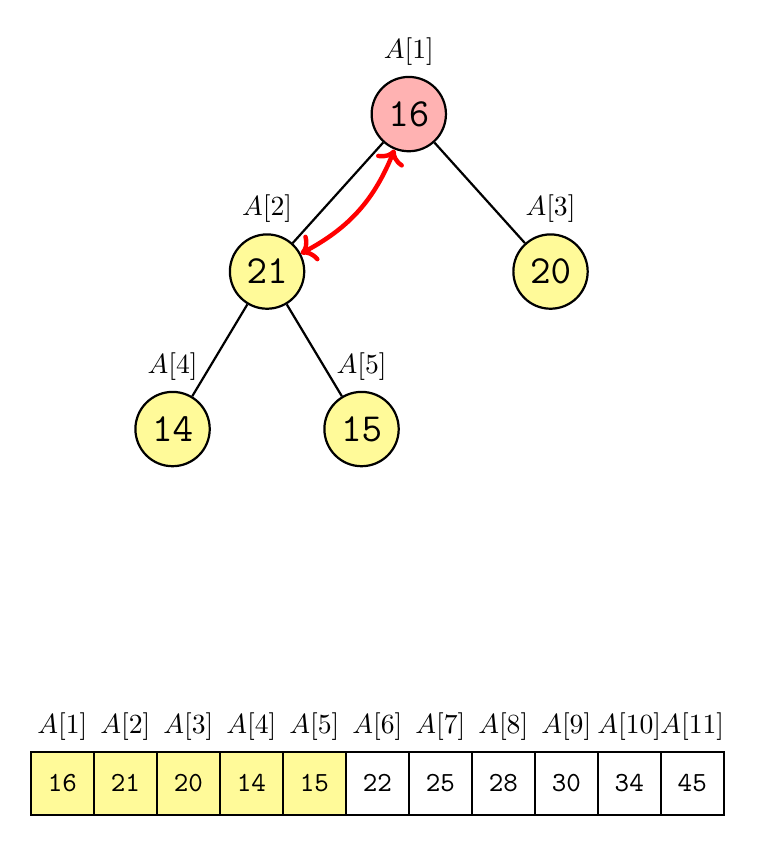
\begin{tikzpicture}[
  thick,
  level distance=2cm,
  level 1/.style={sibling distance=3.6cm},
  level 2/.style={sibling distance=2.4cm},
  level 3/.style={sibling distance=1.2cm},
	font=\ttfamily\bfseries]
  \node[mynoder, minimum size=0.9cm,label={above:$A[1]$}] at (0,0) (a) {16}
    child {node[mynode, minimum size=0.9cm,label={above:$A[2]$}] (b)  {21}
      child {node[mynode, minimum size=0.9cm,label={above:$A[4]$}] {14}}
      child {node[mynode, minimum size=0.9cm,label={above:$A[5]$}]    {15}}
    }
    child {node[mynode, minimum size=0.9cm,label={above:$A[3]$}] {20}}
    ;
    
\node[draw,rectangle,minimum size=0.80cm,label={above:$A[1]$}, fill=yellow!40] at (-4.40,-8.5) {16};
\node[draw,rectangle,minimum size=0.80cm,label={above:$A[2]$}, fill=yellow!40] at (-3.60,-8.5) {21};
\node[draw,rectangle,minimum size=0.80cm,label={above:$A[3]$}, fill=yellow!40] at (-2.80,-8.5) {20};
\node[draw,rectangle,minimum size=0.80cm,label={above:$A[4]$}, fill=yellow!40] at (-2.00,-8.5) {14};
\node[draw,rectangle,minimum size=0.80cm,label={above:$A[5]$}, fill=yellow!40] at (-1.20,-8.5) {15};
\node[draw,rectangle,minimum size=0.80cm,label={above:$A[6]$}] at (-0.40,-8.5) {22};
\node[draw,rectangle,minimum size=0.80cm,label={above:$A[7]$}] at ( 0.40,-8.5) {25};
\node[draw,rectangle,minimum size=0.80cm,label={above:$A[8]$}] at ( 1.20,-8.5) {28};
\node[draw,rectangle,minimum size=0.80cm,label={above:$A[9]$}] at ( 2.00,-8.5) {30};
\node[draw,rectangle,minimum size=0.80cm,label={above:$A[10]$}] at ( 2.80,-8.5) {34};
\node[draw,rectangle,minimum size=0.80cm,label={above:$A[11]$}] at ( 3.60,-8.5) {45};

  \draw[edger,<->] (a) edge[bend left=20] node {} (b);

 \end{tikzpicture}

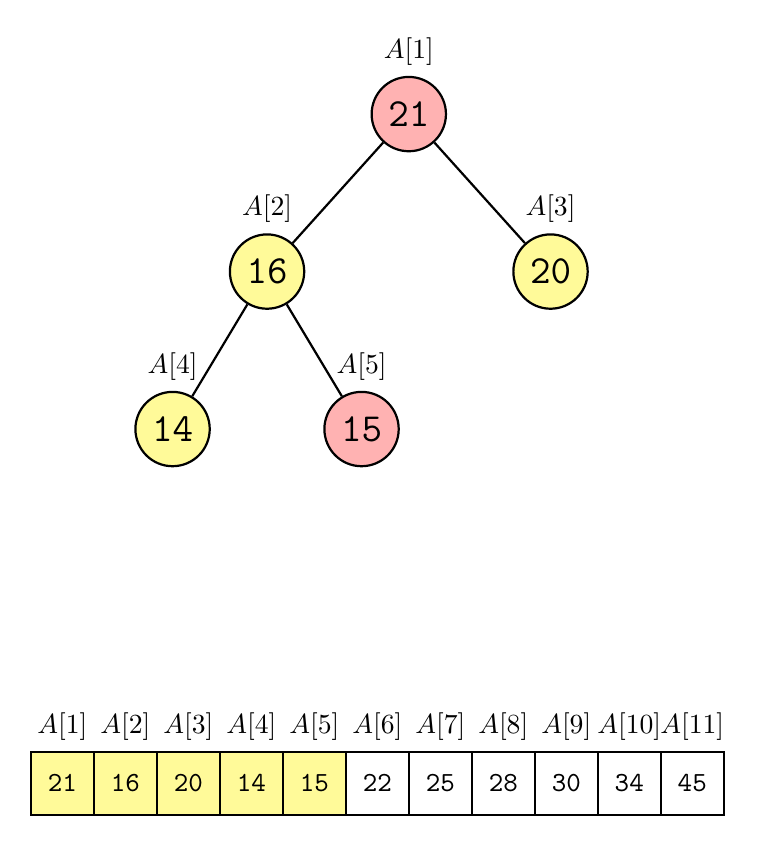
\begin{tikzpicture}[
  thick,
  level distance=2cm,
  level 1/.style={sibling distance=3.6cm},
  level 2/.style={sibling distance=2.4cm},
  level 3/.style={sibling distance=1.2cm},
	font=\ttfamily\bfseries]
  \node[mynoder, minimum size=0.9cm,label={above:$A[1]$}] at (0,0) (a) {21}
    child {node[mynode, minimum size=0.9cm,label={above:$A[2]$}] (b)  {16}
      child {node[mynode, minimum size=0.9cm,label={above:$A[4]$}] {14}}
      child {node[mynoder, minimum size=0.9cm,label={above:$A[5]$}]    {15}}
    }
    child {node[mynode, minimum size=0.9cm,label={above:$A[3]$}] {20}}
    ;
    
\node[draw,rectangle,minimum size=0.80cm,label={above:$A[1]$}, fill=yellow!40] at (-4.40,-8.5) {21};
\node[draw,rectangle,minimum size=0.80cm,label={above:$A[2]$}, fill=yellow!40] at (-3.60,-8.5) {16};
\node[draw,rectangle,minimum size=0.80cm,label={above:$A[3]$}, fill=yellow!40] at (-2.80,-8.5) {20};
\node[draw,rectangle,minimum size=0.80cm,label={above:$A[4]$}, fill=yellow!40] at (-2.00,-8.5) {14};
\node[draw,rectangle,minimum size=0.80cm,label={above:$A[5]$}, fill=yellow!40] at (-1.20,-8.5) {15};
\node[draw,rectangle,minimum size=0.80cm,label={above:$A[6]$}] at (-0.40,-8.5) {22};
\node[draw,rectangle,minimum size=0.80cm,label={above:$A[7]$}] at ( 0.40,-8.5) {25};
\node[draw,rectangle,minimum size=0.80cm,label={above:$A[8]$}] at ( 1.20,-8.5) {28};
\node[draw,rectangle,minimum size=0.80cm,label={above:$A[9]$}] at ( 2.00,-8.5) {30};
\node[draw,rectangle,minimum size=0.80cm,label={above:$A[10]$}] at ( 2.80,-8.5) {34};
\node[draw,rectangle,minimum size=0.80cm,label={above:$A[11]$}] at ( 3.60,-8.5) {45};

 \end{tikzpicture}

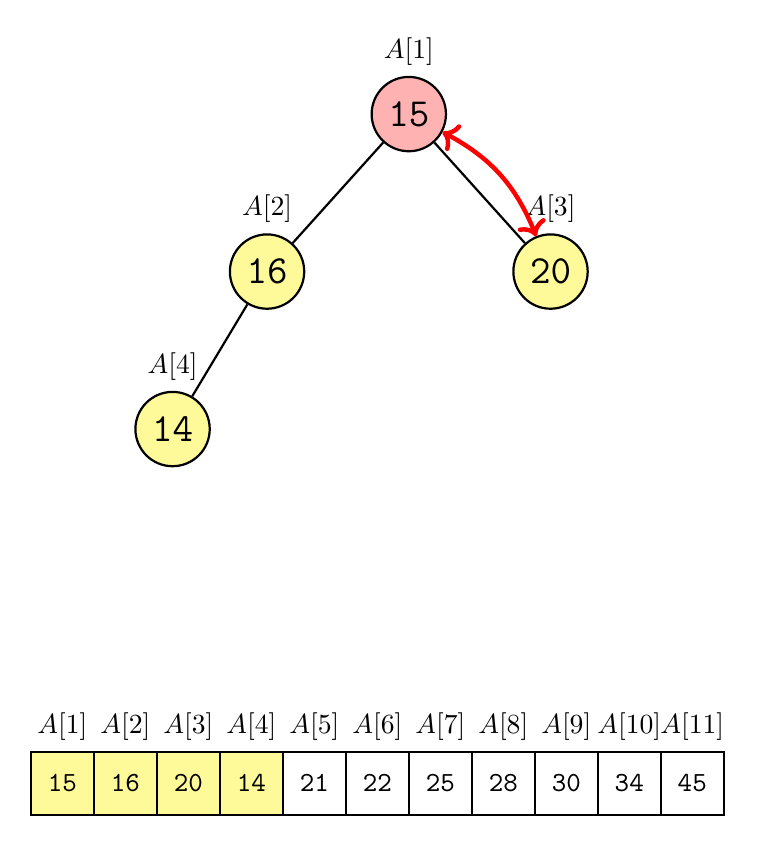
\begin{tikzpicture}[
  thick,
  level distance=2cm,
  level 1/.style={sibling distance=3.6cm},
  level 2/.style={sibling distance=2.4cm},
  level 3/.style={sibling distance=1.2cm},
	font=\ttfamily\bfseries]
  \node[mynoder, minimum size=0.9cm,label={above:$A[1]$}] at (0,0) (a) {15}
    child {node[mynode, minimum size=0.9cm,label={above:$A[2]$}]   {16}
      child {node[mynode, minimum size=0.9cm,label={above:$A[4]$}] {14}}
      child[missing] {node[mynoder, minimum size=0.9cm,label={above:$A[5]$}]    {15}}
    }
    child {node[mynode, minimum size=0.9cm,label={above:$A[3]$}] (b) {20}}
    ;
    
\node[draw,rectangle,minimum size=0.80cm,label={above:$A[1]$}, fill=yellow!40] at (-4.40,-8.5) {15};
\node[draw,rectangle,minimum size=0.80cm,label={above:$A[2]$}, fill=yellow!40] at (-3.60,-8.5) {16};
\node[draw,rectangle,minimum size=0.80cm,label={above:$A[3]$}, fill=yellow!40] at (-2.80,-8.5) {20};
\node[draw,rectangle,minimum size=0.80cm,label={above:$A[4]$}, fill=yellow!40] at (-2.00,-8.5) {14};
\node[draw,rectangle,minimum size=0.80cm,label={above:$A[5]$}] at (-1.20,-8.5) {21};
\node[draw,rectangle,minimum size=0.80cm,label={above:$A[6]$}] at (-0.40,-8.5) {22};
\node[draw,rectangle,minimum size=0.80cm,label={above:$A[7]$}] at ( 0.40,-8.5) {25};
\node[draw,rectangle,minimum size=0.80cm,label={above:$A[8]$}] at ( 1.20,-8.5) {28};
\node[draw,rectangle,minimum size=0.80cm,label={above:$A[9]$}] at ( 2.00,-8.5) {30};
\node[draw,rectangle,minimum size=0.80cm,label={above:$A[10]$}] at ( 2.80,-8.5) {34};
\node[draw,rectangle,minimum size=0.80cm,label={above:$A[11]$}] at ( 3.60,-8.5) {45};

  \draw[edger,<->] (a) edge[bend left=20] node {} (b);

 \end{tikzpicture}

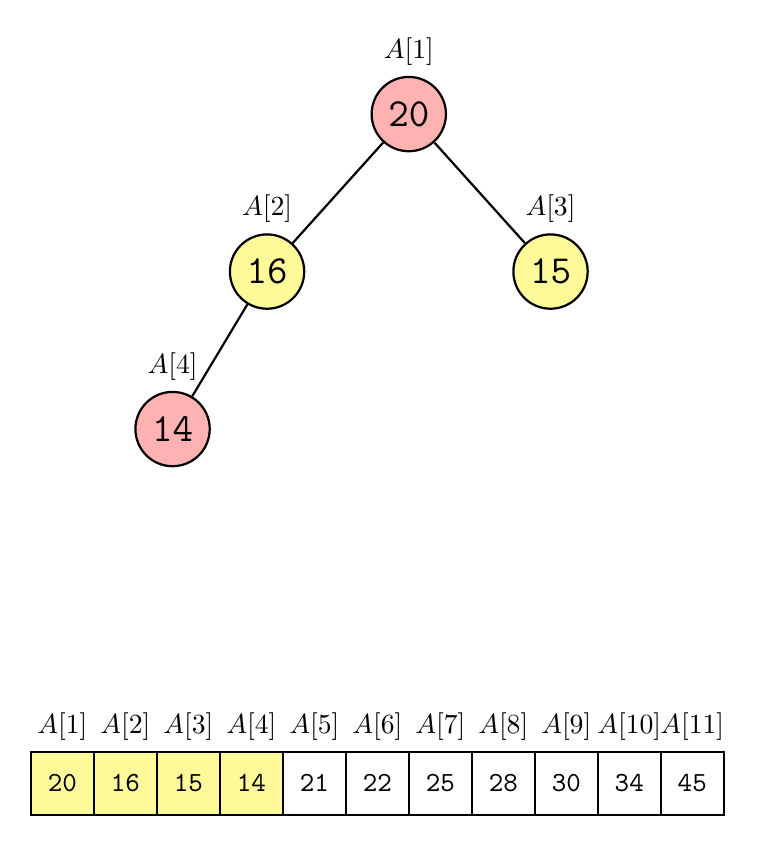
\begin{tikzpicture}[
  thick,
  level distance=2cm,
  level 1/.style={sibling distance=3.6cm},
  level 2/.style={sibling distance=2.4cm},
  level 3/.style={sibling distance=1.2cm},
	font=\ttfamily\bfseries]
  \node[mynoder, minimum size=0.9cm,label={above:$A[1]$}] at (0,0) (a) {20}
    child {node[mynode, minimum size=0.9cm,label={above:$A[2]$}]   {16}
      child {node[mynoder, minimum size=0.9cm,label={above:$A[4]$}] {14}}
      child[missing] {node[mynoder, minimum size=0.9cm,label={above:$A[5]$}]    {}}
    }
    child {node[mynode, minimum size=0.9cm,label={above:$A[3]$}] (b) {15}}
    ;
    
\node[draw,rectangle,minimum size=0.80cm,label={above:$A[1]$}, fill=yellow!40] at (-4.40,-8.5) {20};
\node[draw,rectangle,minimum size=0.80cm,label={above:$A[2]$}, fill=yellow!40] at (-3.60,-8.5) {16};
\node[draw,rectangle,minimum size=0.80cm,label={above:$A[3]$}, fill=yellow!40] at (-2.80,-8.5) {15};
\node[draw,rectangle,minimum size=0.80cm,label={above:$A[4]$}, fill=yellow!40] at (-2.00,-8.5) {14};
\node[draw,rectangle,minimum size=0.80cm,label={above:$A[5]$}] at (-1.20,-8.5) {21};
\node[draw,rectangle,minimum size=0.80cm,label={above:$A[6]$}] at (-0.40,-8.5) {22};
\node[draw,rectangle,minimum size=0.80cm,label={above:$A[7]$}] at ( 0.40,-8.5) {25};
\node[draw,rectangle,minimum size=0.80cm,label={above:$A[8]$}] at ( 1.20,-8.5) {28};
\node[draw,rectangle,minimum size=0.80cm,label={above:$A[9]$}] at ( 2.00,-8.5) {30};
\node[draw,rectangle,minimum size=0.80cm,label={above:$A[10]$}] at ( 2.80,-8.5) {34};
\node[draw,rectangle,minimum size=0.80cm,label={above:$A[11]$}] at ( 3.60,-8.5) {45};


 \end{tikzpicture}


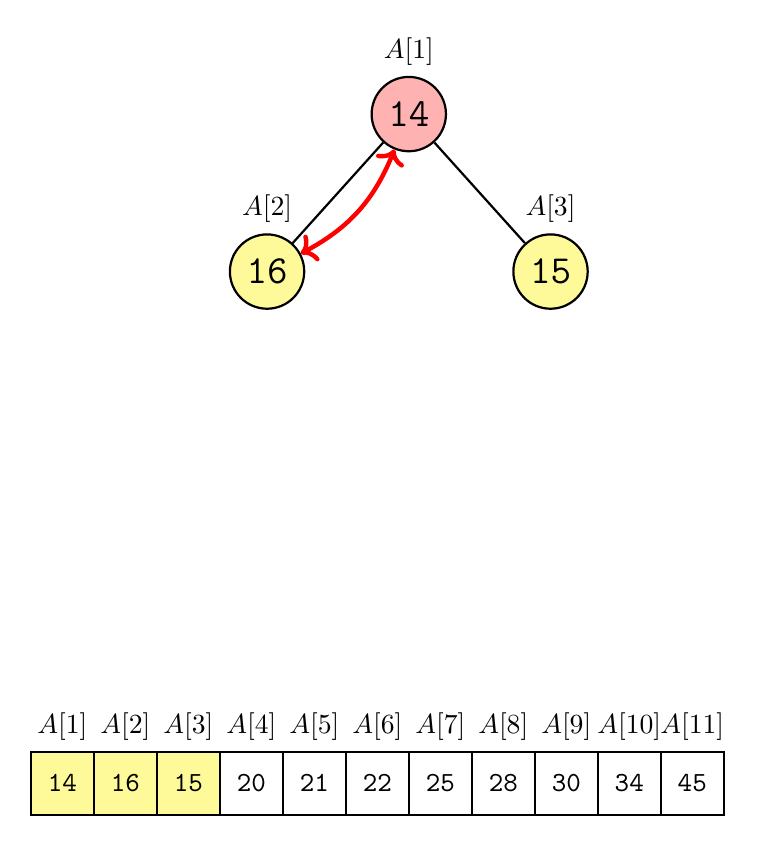
\begin{tikzpicture}[
  thick,
  level distance=2cm,
  level 1/.style={sibling distance=3.6cm},
  level 2/.style={sibling distance=2.4cm},
  level 3/.style={sibling distance=1.2cm},
	font=\ttfamily\bfseries]
  \node[mynoder, minimum size=0.9cm,label={above:$A[1]$}] at (0,0) (a) {14}
    child {node[mynode, minimum size=0.9cm,label={above:$A[2]$}] (b)  {16} }
    child {node[mynode, minimum size=0.9cm,label={above:$A[3]$}] {15}}
    ;
    
\node[draw,rectangle,minimum size=0.80cm,label={above:$A[1]$}, fill=yellow!40] at (-4.40,-8.5) {14};
\node[draw,rectangle,minimum size=0.80cm,label={above:$A[2]$}, fill=yellow!40] at (-3.60,-8.5) {16};
\node[draw,rectangle,minimum size=0.80cm,label={above:$A[3]$}, fill=yellow!40] at (-2.80,-8.5) {15};
\node[draw,rectangle,minimum size=0.80cm,label={above:$A[4]$}] at (-2.00,-8.5) {20};
\node[draw,rectangle,minimum size=0.80cm,label={above:$A[5]$}] at (-1.20,-8.5) {21};
\node[draw,rectangle,minimum size=0.80cm,label={above:$A[6]$}] at (-0.40,-8.5) {22};
\node[draw,rectangle,minimum size=0.80cm,label={above:$A[7]$}] at ( 0.40,-8.5) {25};
\node[draw,rectangle,minimum size=0.80cm,label={above:$A[8]$}] at ( 1.20,-8.5) {28};
\node[draw,rectangle,minimum size=0.80cm,label={above:$A[9]$}] at ( 2.00,-8.5) {30};
\node[draw,rectangle,minimum size=0.80cm,label={above:$A[10]$}] at ( 2.80,-8.5) {34};
\node[draw,rectangle,minimum size=0.80cm,label={above:$A[11]$}] at ( 3.60,-8.5) {45};

  \draw[edger,<->] (a) edge[bend left=20] node {} (b);


 \end{tikzpicture}

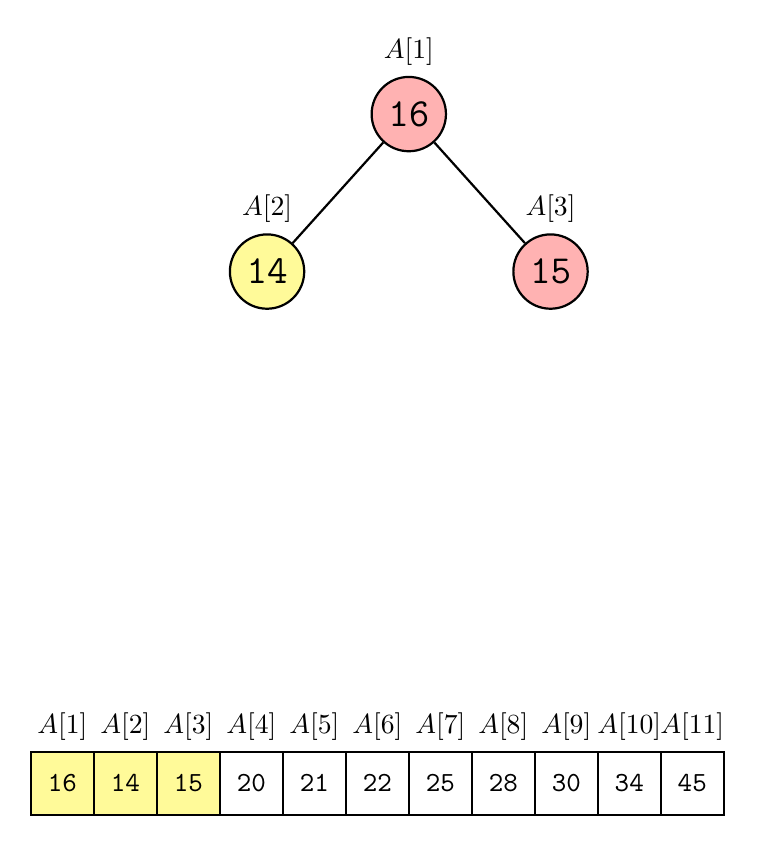
\begin{tikzpicture}[
  thick,
  level distance=2cm,
  level 1/.style={sibling distance=3.6cm},
  level 2/.style={sibling distance=2.4cm},
  level 3/.style={sibling distance=1.2cm},
	font=\ttfamily\bfseries]
  \node[mynoder, minimum size=0.9cm,label={above:$A[1]$}] at (0,0) (a) {16}
    child {node[mynode, minimum size=0.9cm,label={above:$A[2]$}] (b)  {14} }
    child {node[mynoder, minimum size=0.9cm,label={above:$A[3]$}] {15}}
    ;
    
\node[draw,rectangle,minimum size=0.80cm,label={above:$A[1]$}, fill=yellow!40] at (-4.40,-8.5) {16};
\node[draw,rectangle,minimum size=0.80cm,label={above:$A[2]$}, fill=yellow!40] at (-3.60,-8.5) {14};
\node[draw,rectangle,minimum size=0.80cm,label={above:$A[3]$}, fill=yellow!40] at (-2.80,-8.5) {15};
\node[draw,rectangle,minimum size=0.80cm,label={above:$A[4]$}] at (-2.00,-8.5) {20};
\node[draw,rectangle,minimum size=0.80cm,label={above:$A[5]$}] at (-1.20,-8.5) {21};
\node[draw,rectangle,minimum size=0.80cm,label={above:$A[6]$}] at (-0.40,-8.5) {22};
\node[draw,rectangle,minimum size=0.80cm,label={above:$A[7]$}] at ( 0.40,-8.5) {25};
\node[draw,rectangle,minimum size=0.80cm,label={above:$A[8]$}] at ( 1.20,-8.5) {28};
\node[draw,rectangle,minimum size=0.80cm,label={above:$A[9]$}] at ( 2.00,-8.5) {30};
\node[draw,rectangle,minimum size=0.80cm,label={above:$A[10]$}] at ( 2.80,-8.5) {34};
\node[draw,rectangle,minimum size=0.80cm,label={above:$A[11]$}] at ( 3.60,-8.5) {45};

 % \draw[edger,<->] (a) edge[bend left=20] node {} (b);


 \end{tikzpicture}

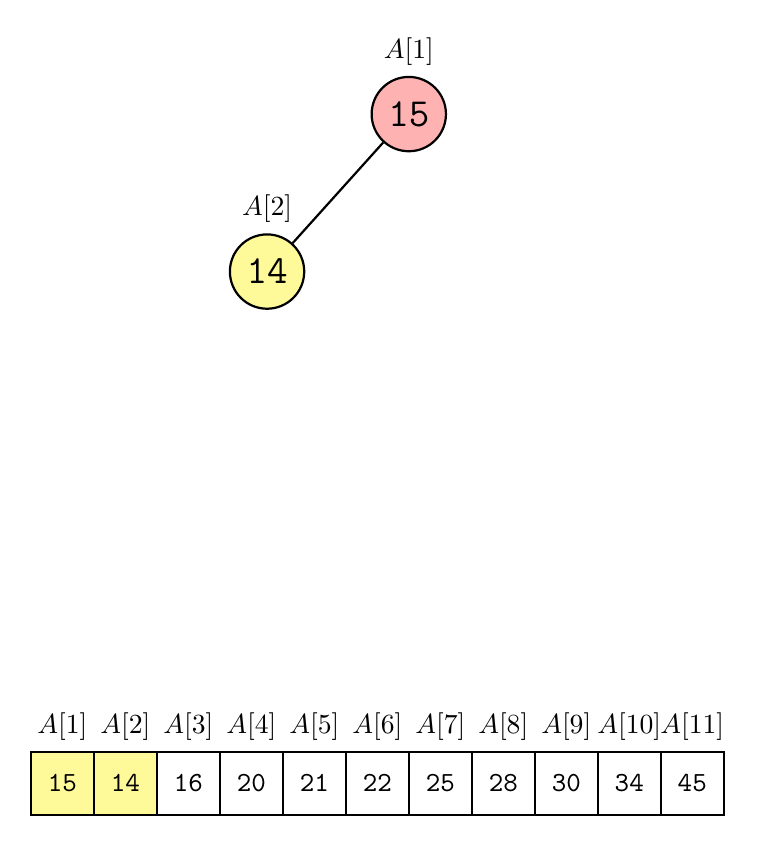
\begin{tikzpicture}[
  thick,
  level distance=2cm,
  level 1/.style={sibling distance=3.6cm},
  level 2/.style={sibling distance=2.4cm},
  level 3/.style={sibling distance=1.2cm},
	font=\ttfamily\bfseries]
  \node[mynoder, minimum size=0.9cm,label={above:$A[1]$}] at (0,0) (a) {15}
    child {node[mynode, minimum size=0.9cm,label={above:$A[2]$}] (b)  {14} }
    child[missing] {node[mynoder, minimum size=0.9cm,label={above:$A[3]$}] {}}
    ;
    
\node[draw,rectangle,minimum size=0.80cm,label={above:$A[1]$}, fill=yellow!40] at (-4.40,-8.5) {15};
\node[draw,rectangle,minimum size=0.80cm,label={above:$A[2]$}, fill=yellow!40] at (-3.60,-8.5) {14};
\node[draw,rectangle,minimum size=0.80cm,label={above:$A[3]$}] at (-2.80,-8.5) {16};
\node[draw,rectangle,minimum size=0.80cm,label={above:$A[4]$}] at (-2.00,-8.5) {20};
\node[draw,rectangle,minimum size=0.80cm,label={above:$A[5]$}] at (-1.20,-8.5) {21};
\node[draw,rectangle,minimum size=0.80cm,label={above:$A[6]$}] at (-0.40,-8.5) {22};
\node[draw,rectangle,minimum size=0.80cm,label={above:$A[7]$}] at ( 0.40,-8.5) {25};
\node[draw,rectangle,minimum size=0.80cm,label={above:$A[8]$}] at ( 1.20,-8.5) {28};
\node[draw,rectangle,minimum size=0.80cm,label={above:$A[9]$}] at ( 2.00,-8.5) {30};
\node[draw,rectangle,minimum size=0.80cm,label={above:$A[10]$}] at ( 2.80,-8.5) {34};
\node[draw,rectangle,minimum size=0.80cm,label={above:$A[11]$}] at ( 3.60,-8.5) {45};

% \draw[edger,<->] (a) edge[bend left=20] node {} (b);


 \end{tikzpicture}

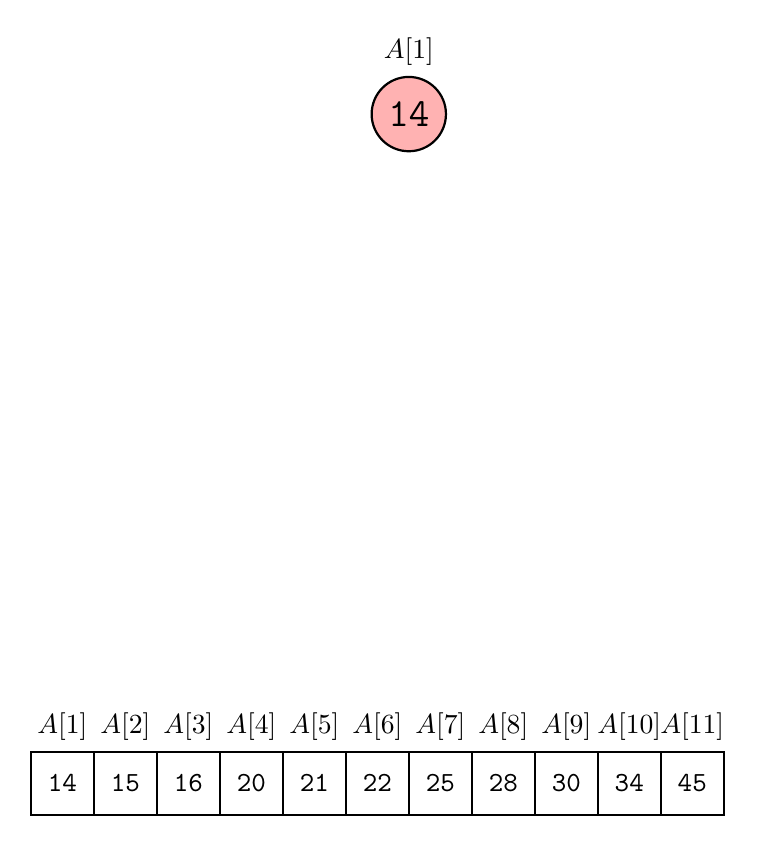
\begin{tikzpicture}[
  thick,
  level distance=2cm,
  level 1/.style={sibling distance=3.6cm},
  level 2/.style={sibling distance=2.4cm},
  level 3/.style={sibling distance=1.2cm},
	font=\ttfamily\bfseries]
  \node[mynoder, minimum size=0.9cm,label={above:$A[1]$}] at (0,0) (a) {14}
    ;
    
\node[draw,rectangle,minimum size=0.80cm,label={above:$A[1]$}] at (-4.40,-8.5) {14};
\node[draw,rectangle,minimum size=0.80cm,label={above:$A[2]$}] at (-3.60,-8.5) {15};
\node[draw,rectangle,minimum size=0.80cm,label={above:$A[3]$}] at (-2.80,-8.5) {16};
\node[draw,rectangle,minimum size=0.80cm,label={above:$A[4]$}] at (-2.00,-8.5) {20};
\node[draw,rectangle,minimum size=0.80cm,label={above:$A[5]$}] at (-1.20,-8.5) {21};
\node[draw,rectangle,minimum size=0.80cm,label={above:$A[6]$}] at (-0.40,-8.5) {22};
\node[draw,rectangle,minimum size=0.80cm,label={above:$A[7]$}] at ( 0.40,-8.5) {25};
\node[draw,rectangle,minimum size=0.80cm,label={above:$A[8]$}] at ( 1.20,-8.5) {28};
\node[draw,rectangle,minimum size=0.80cm,label={above:$A[9]$}] at ( 2.00,-8.5) {30};
\node[draw,rectangle,minimum size=0.80cm,label={above:$A[10]$}] at ( 2.80,-8.5) {34};
\node[draw,rectangle,minimum size=0.80cm,label={above:$A[11]$}] at ( 3.60,-8.5) {45};

% \draw[edger,<->] (a) edge[bend left=20] node {} (b);


 \end{tikzpicture}


\end{document}
